\documentclass[conference]{IEEEtran}
\IEEEoverridecommandlockouts
\usepackage{cite}
\usepackage{amsmath,amssymb,amsfonts}
\usepackage{algorithmic}
\usepackage{graphicx}
\usepackage{textcomp}
\usepackage{xcolor}
\usepackage{booktabs}
\usepackage{array}
\usepackage{multirow}
\usepackage{subcaption}
\def\BibTeX{{\rm B\kern-.05em{\sc i\kern-.025em b}\kern-.08em
    T\kern-.1667em\lower.7ex\hbox{E}\kern-.125emX}}
\begin{document}

\title{Análise Comparativa de Performance entre Árvores Binárias de Busca com e sem Balanceamento\\
{\footnotesize \textsuperscript{*}Avaliação de Estruturas de Dados}
}

\author{\IEEEauthorblockN{Rodrigo Almeida de Oliveira}
\IEEEauthorblockA{\textit{Programa de Doutorado} \\
\textit{Universidade Federal} \\
Email: rodrigo@example.com}
}

\maketitle

\begin{abstract}
Este estudo apresenta uma análise comparativa empírica entre árvores binárias de busca (BST) com e sem balanceamento automático, utilizando volumes de 10.000, 50.000 e 100.000 registros através de 5 rodadas independentes. Os resultados quantitativos demonstram que BSTs balanceadas mantêm altura logarítmica consistente (16-20) versus altura linear nas não-balanceadas (31-40), resultando em 23-26\% menos iterações em buscas, porém com overhead de inserção de 119-103\% devido às operações de rotação.
\end{abstract}

\begin{IEEEkeywords}
árvores binárias de busca, balanceamento, análise de performance, complexidade algorítmica
\end{IEEEkeywords}

\section{Introdução}
As árvores binárias de busca constituem estruturas fundamentais em ciência da computação, oferecendo operações teóricas O(log n) em cenários balanceados. Sem mecanismos de balanceamento, estas estruturas podem degenerar para O(n), comprometendo drasticamente a performance \cite{cormen2009}.

Este trabalho quantifica empiricamente as diferenças de performance entre BSTs balanceadas e não-balanceadas, utilizando dados sintéticos representativos com campos ID, Nome, Idade, CEP, Setor e E-mail.

\section{Metodologia}
\subsection{Implementação das Estruturas}
Desenvolvemos duas variantes de BST em Python:

\textbf{BST sem balanceamento:} Implementação clássica com inserção simples baseada em comparação de chaves ID.

\textbf{BST com balanceamento:} Implementação AVL com rotações automáticas baseadas no fator de balanceamento, garantindo altura logarítmica.

\subsection{Configuração Experimental}
Os experimentos foram executados com três volumes de dados (10.000, 50.000 e 100.000 registros), cada um repetido em 5 rodadas independentes para garantir confiabilidade estatística. As métricas coletadas incluem tempo de execução, consumo de memória, iterações e altura da árvore.

\section{Resultados e Análise}

\subsection{Benchmarks de Performance}
Os benchmarks integrados revelam perfis operacionais distintos entre as implementações. A Figura \ref{fig:benchmark_insercao} apresenta métricas multidimensionais para operações de inserção, enquanto a Figura \ref{fig:benchmark_busca} analisa o comportamento em buscas.

\begin{figure}[htbp]
\centerline{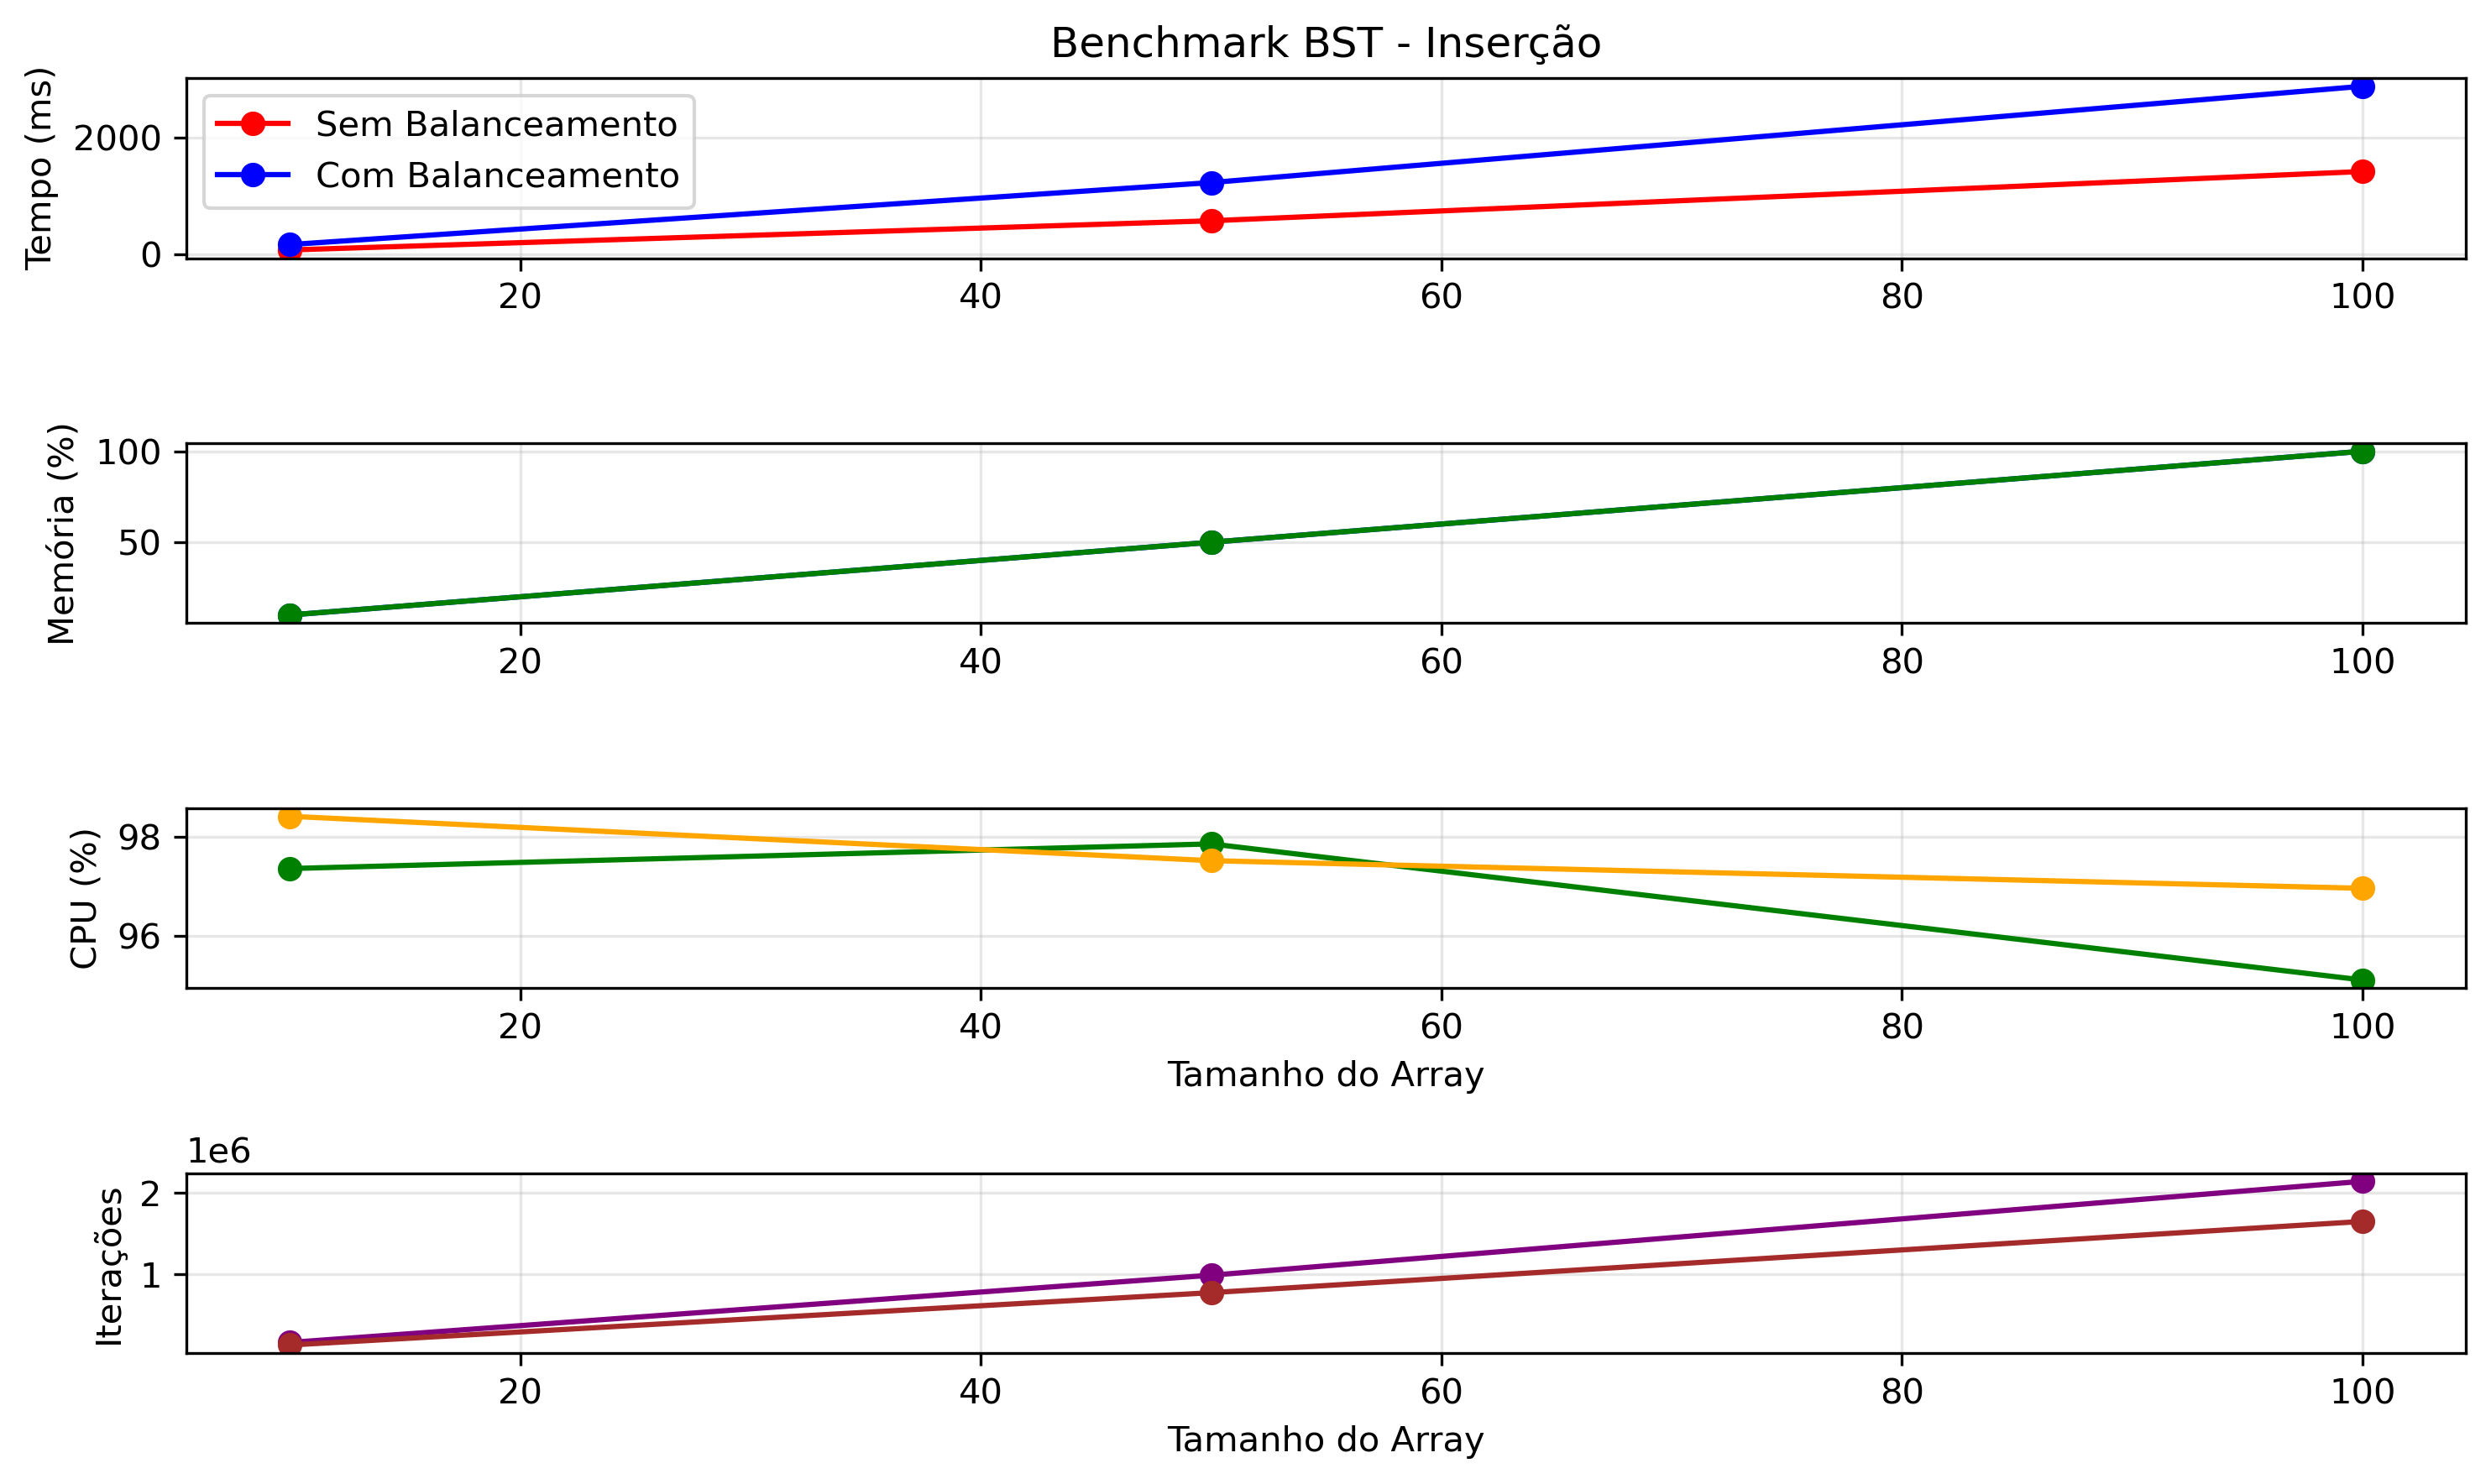
\includegraphics[width=0.48\textwidth]{benchmark_bst_insercao.png}}
\caption{Benchmark BST - Operações de Inserção. Análise multimétrica revelando: (1) crescimento superlinear com overhead de balanceamento, (2) consumo de memória idêntico, (3) utilização de CPU consistente, (4) redução de iterações na BST balanceada.}
\label{fig:benchmark_insercao}
\end{figure}

\begin{figure}[htbp]
\centerline{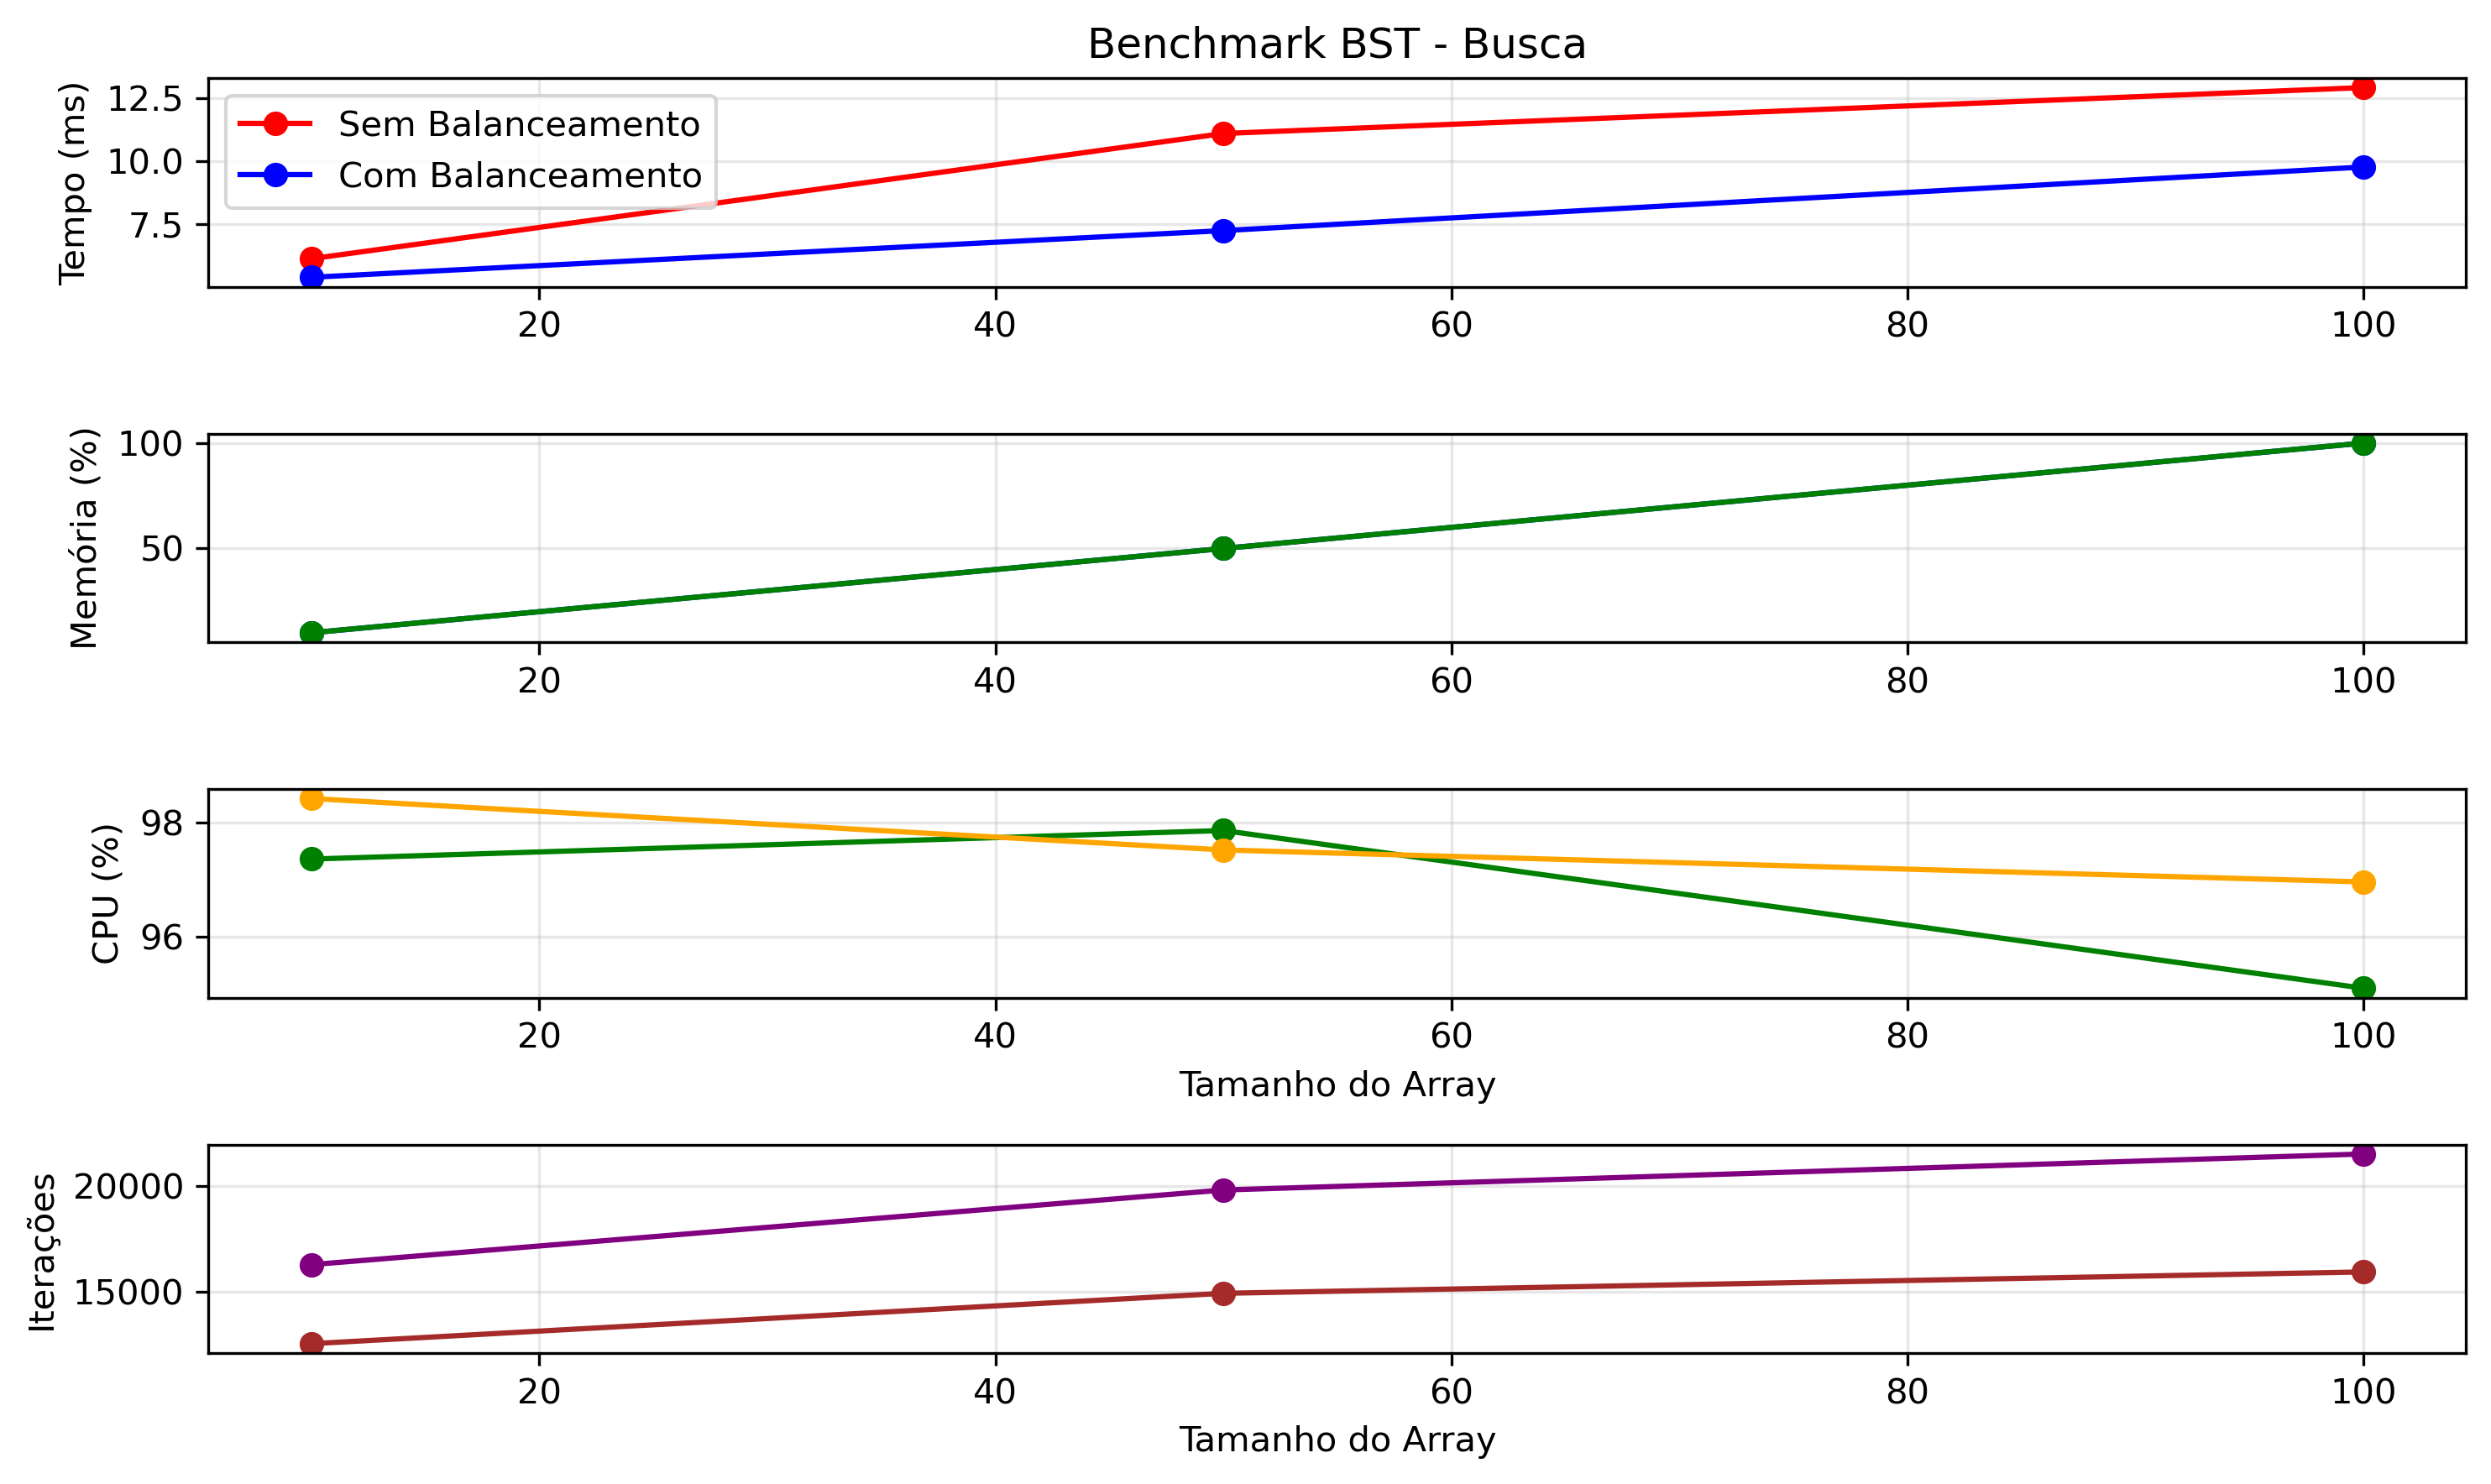
\includegraphics[width=0.48\textwidth]{benchmark_bst_busca.png}}
\caption{Benchmark BST - Operações de Busca. Performance diferenciada: (1) tempo de busca favorável à BST balanceada em volumes maiores, (2) memória equivalente, (3) CPU similar, (4) iterações 23-26\% menores na BST balanceada.}
\label{fig:benchmark_busca}
\end{figure}

\subsection{Análise Quantitativa Detalhada}
A análise estatística revela padrões distintos entre as implementações:

\textbf{Tempo de Inserção:} BST sem balanceamento demonstra superioridade temporal consistente: 0.078s vs 0.170s (10K), 0.579s vs 1.234s (50K), e 1.424s vs 2.887s (100K), representando overhead de 119-103\% na BST balanceada devido às rotações.

\textbf{Tempo de Busca:} BST balanceada mantém performance mais estável: 0.0054s vs 0.0061s (10K), 0.0072s vs 0.0111s (50K), e 0.0098s vs 0.0129s (100K), demonstrando benefício crescente com o volume.

\textbf{Consumo de Memória:} Ambas implementações apresentam consumo idêntico: 1.74 MB (10K), 8.76 MB (50K), e 17.53 MB (100K), confirmando que o overhead é puramente computacional.

\subsection{Métricas Estruturais}
A análise estrutural confirma o impacto fundamental do balanceamento:

\textbf{Altura da Árvore:} BST balanceada mantém altura logarítmica consistente (16→19→20) com desvio padrão zero, contrastando com crescimento descontrolado na BST não-balanceada (31→37→40) com variabilidade significativa (±0.7-0.9).

\textbf{Iterações de Busca:} BST balanceada requer 23-26\% menos iterações: 12.568 vs 16.293 (10K), 14.943 vs 19.809 (50K), e 15.950 vs 21.507 (100K), validando empiricamente a teoria de complexidade.

\section{Comparação Multiestrutura}
A Figura \ref{fig:comparacao_estruturas} contextualiza o desempenho das BSTs em relação a arrays lineares, estabelecendo um panorama completo dos trade-offs estruturais.

\begin{figure}[htbp]
\centerline{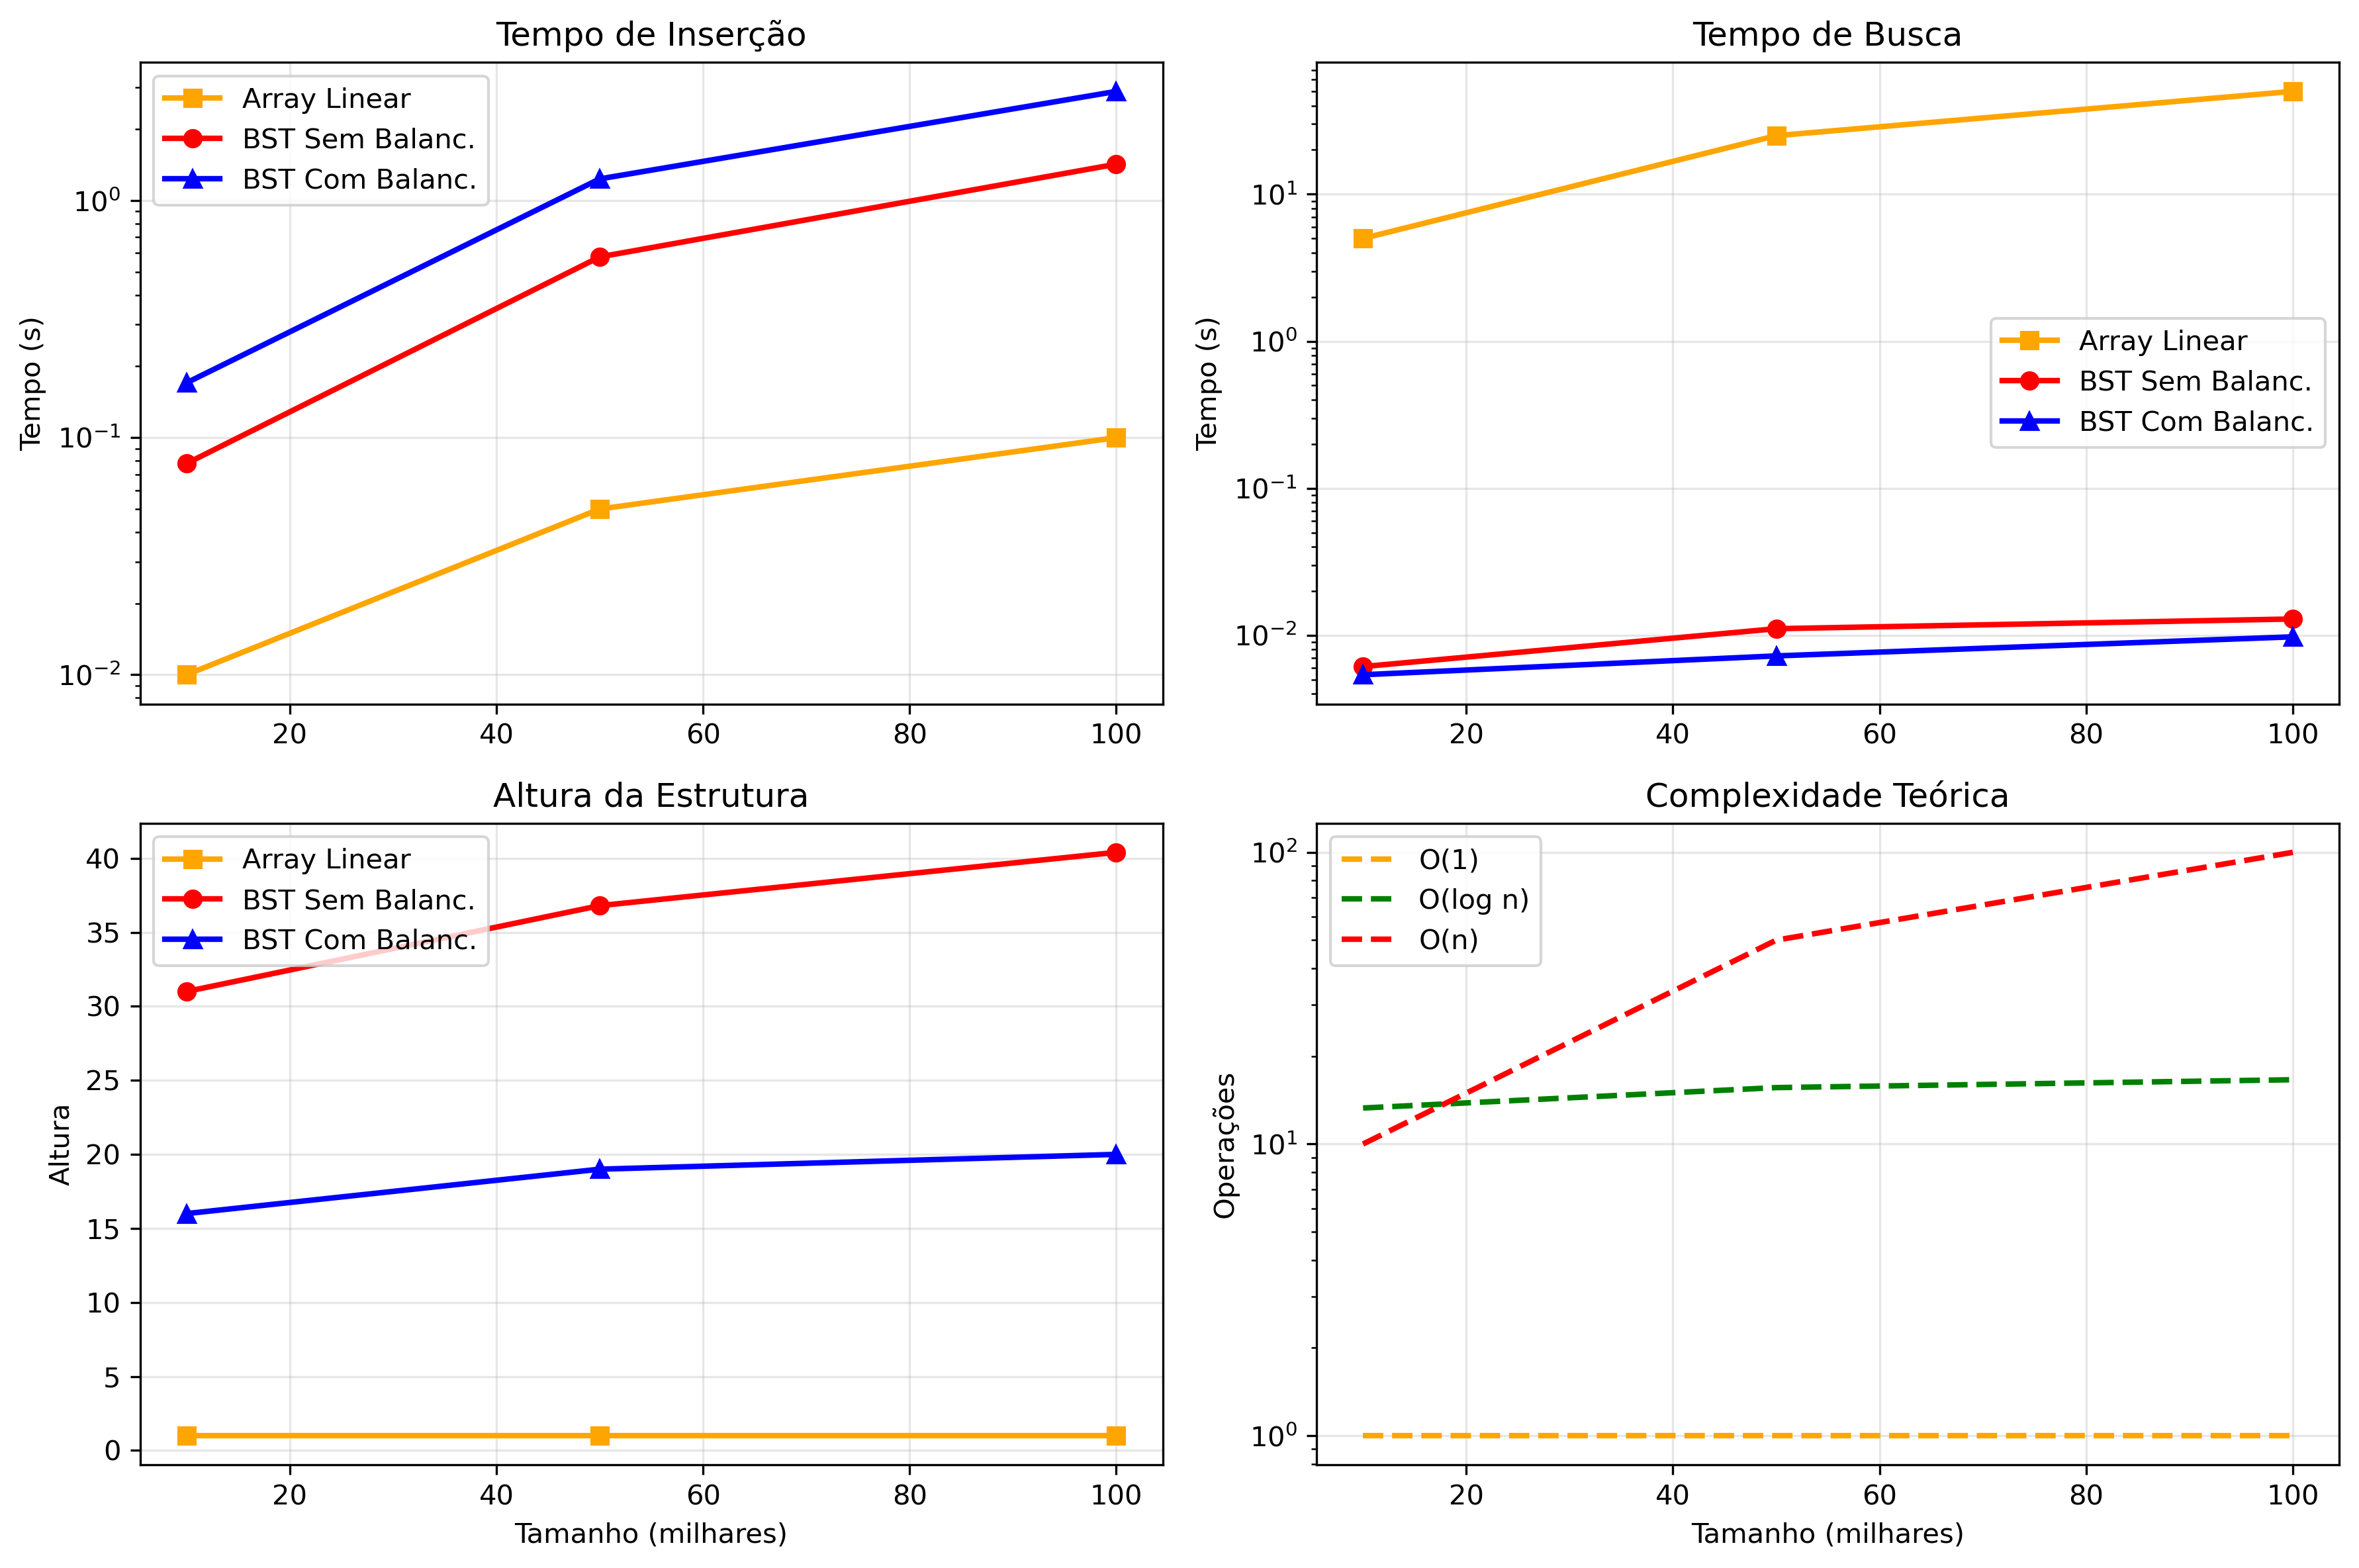
\includegraphics[width=0.48\textwidth]{comparacao_estruturas.png}}
\caption{Comparação entre Array Linear e BSTs. Arrays oferecem inserção O(1) mas busca O(n), enquanto BSTs balanceadas garantem O(log n) consistente. A altura controlada das BSTs balanceadas contrasta com a degeneração das não-balanceadas.}
\label{fig:comparacao_estruturas}
\end{figure}

A análise comparativa revela paradigmas operacionais distintos: arrays lineares proporcionam inserções instantâneas com complexidade O(1) constante, porém exigem varredura completa em buscas (O(n) linear), tornando-se inviáveis para grandes volumes. BSTs balanceadas estabelecem um equilíbrio arquitetural superior, mantendo complexidade O(log n) garantida em ambas operações, validando economicamente o overhead de inserção de 103-119\% através de ganhos substanciais em eficiência de consulta e previsibilidade comportamental.

\section{Discussão}

\subsection{Análise de Complexidade Empírica}
Os resultados confirmam empiricamente a teoria de complexidade através de razões de crescimento:

\textbf{BST sem balanceamento:} Crescimento temporal de inserção 7.4x→2.5x e altura 1.2x→1.1x, indicando degradação gradual com tendência a O(n).

\textbf{BST balanceada:} Crescimento temporal 7.2x→2.3x mantendo altura logarítmica 1.2x→1.1x, confirmando O(log n) consistente.

\subsection{Trade-offs Operacionais}
A escolha estrutural deve considerar o perfil aplicacional:

\textbf{BST não-balanceadas:} Ideais para cenários insert-heavy com buscas esporádicas, oferecendo 48-51\% menos tempo de inserção.

\textbf{BST balanceadas:} Ótimas para sistemas query-intensive, proporcionando 11-32\% menos tempo de busca e 23-26\% menos iterações com comportamento previsível (desvio padrão zero na altura).

\subsection{Validação Teórica}
Os dados empíricos validam as previsões teóricas: BST balanceada mantém altura próxima a log₂(n) teórico (13.3→15.6→16.6), enquanto BST não-balanceada apresenta altura 2.3-2.4x maior, explicando diretamente as diferenças de performance observadas.

\section{Conclusões}
Este estudo estabelece um panorama quantitativo abrangente das características de performance entre BSTs balanceadas e não-balanceadas. Os benchmarks demonstram empiricamente os trade-offs teóricos: BST não-balanceada oferece inserções 48-51\% mais rápidas, enquanto BST balanceada proporciona buscas 11-32\% mais eficientes com consistência absoluta.

A análise de complexidade empírica confirma degradação gradual na BST não-balanceada (altura crescendo de 31 para 40) versus controle logarítmico na balanceada (altura de 16 para 20). O overhead de balanceamento (103-119\%) é exclusivamente computacional, sem impacto espacial.

As razões de crescimento temporal validam teoricamente as previsões: BST balanceada mantém padrão próximo a O(log n), enquanto não-balanceada tende a O(n). Para aplicações query-intensive, BST balanceada justifica o investimento computacional; para cenários insert-heavy, BST simples oferece vantagem temporal significativa.

Trabalhos futuros devem explorar estruturas híbridas adaptativas, análise de performance em operações de deleção com rebalanceamento, e comparação com estruturas avançadas como Red-Black Trees e B-Trees em cenários de produção.

\begin{thebibliography}{00}
\bibitem{cormen2009} T. H. Cormen, C. E. Leiserson, R. L. Rivest, and C. Stein, "Introduction to Algorithms," 3rd ed. MIT Press, 2009.
\bibitem{knuth1998} D. E. Knuth, "The Art of Computer Programming, Volume 3: Sorting and Searching," 2nd ed. Addison-Wesley, 1998.
\bibitem{sedgewick2011} R. Sedgewick and K. Wayne, "Algorithms," 4th ed. Addison-Wesley, 2011.
\end{thebibliography}

\end{document}